\subsection{Interesting Basic Blocks}
We look at three basic blocks where some of the evaluated models behave poorly.
These results are from Haswell.
Table~\ref{tab:case-study} shows these basic blocks, their 
measured throughput, and the throughput predicted by different models.
We manually inspected the instruction schedules predicted by the models
(except for Ithemal, which just predicts a single throughput number).
The first two examples highlight cases of some models' prediction
contradicting instruction throughput specified by the manual.
The last example shows a case where a model (llvm-mca~\cite{llvm-mca} in this case) can significantly
mispredict throughput due to mis-scheduling micro-ops, despite correct modeling of individual instructions.

\textbf{Modelling bug due to unsigned division}.
We look at the first example in Table~\ref{tab:case-study},
which is bottlenecked by a 64-bit by 32-bit unsigned division.
Intel's manual~\cite{intel-manual} states that the throughput of such division
ranges approximately from 20 to 26 cycles, which is consistent with our measurement (21.62).
All models are wrong here; llvm-mca and IACA~\cite{iaca} significantly over-predict;
Ithemal~\cite{ithemal} and OSACA~\cite{osaca} under-predict.
llvm-mca and IACA's predictions indicate that they are confusing 
this division (\verb|div %ecx|) with the 128-bit by 64-bit analog (\verb|div %rcx|),
which the manual does specify to have variable latency between 80 and 95 cycles.
We note that the predictions made by llvm-mca and IACA would still be wrong
were we to replace the \verb|div %ecx| with \verb|div %rcx| in this context,
due to the fast-path for zeroed out \verb|%rdx|.
(which is always the case here because of the preceding \verb|xor %edx, %edx|).

\textbf{Modelling bug due to zero-idioms}.
We look at the second example in Table~\ref{tab:case-study}.
The basic block consists of a single vectorized XOR of \verb|%xmm2| with itself.
All three micro-architectures we evaluated have fast-paths for such zero-idioms. 
IACA and Ithemal recognize this idiom and make predictions close to the measured throughput,
while llvm-mca and OSACA treat this instruction as a regular vectorized XOR.

\textbf{Modeling bug due to mis-scheduling}
The last example in Table~\ref{tab:case-study} is the same basic block
we used as the motivating example in Section~\ref{sec:mapping}.
We focus on the schedule predicted by llvm-mca~\cite{llvm-mca}
and explain why llvm-mca overpredicts.
Figure~\ref{fig:schedule} shows the schedules predicted by llvm-mca and IACA.
Notice that the \verb|xorb| is dispatched for execution noticeably earlier in IACA's schedule.
llvm-mca delays the dispatch of this \verb|xorb| due to its dependence on the previous \verb|xorq|.
llvm-mca is unable to recognize that 
\verb|xorb -1(%rdi), %al| is implemented with a load micro-op followed by an ALU micro-op.
Since the load is independent, the hardware is able to schedule it ahead of time,
hiding its latency completely.
IACA is able to use this fact and predicts accurately.

\begin{figure}[htbp!]
    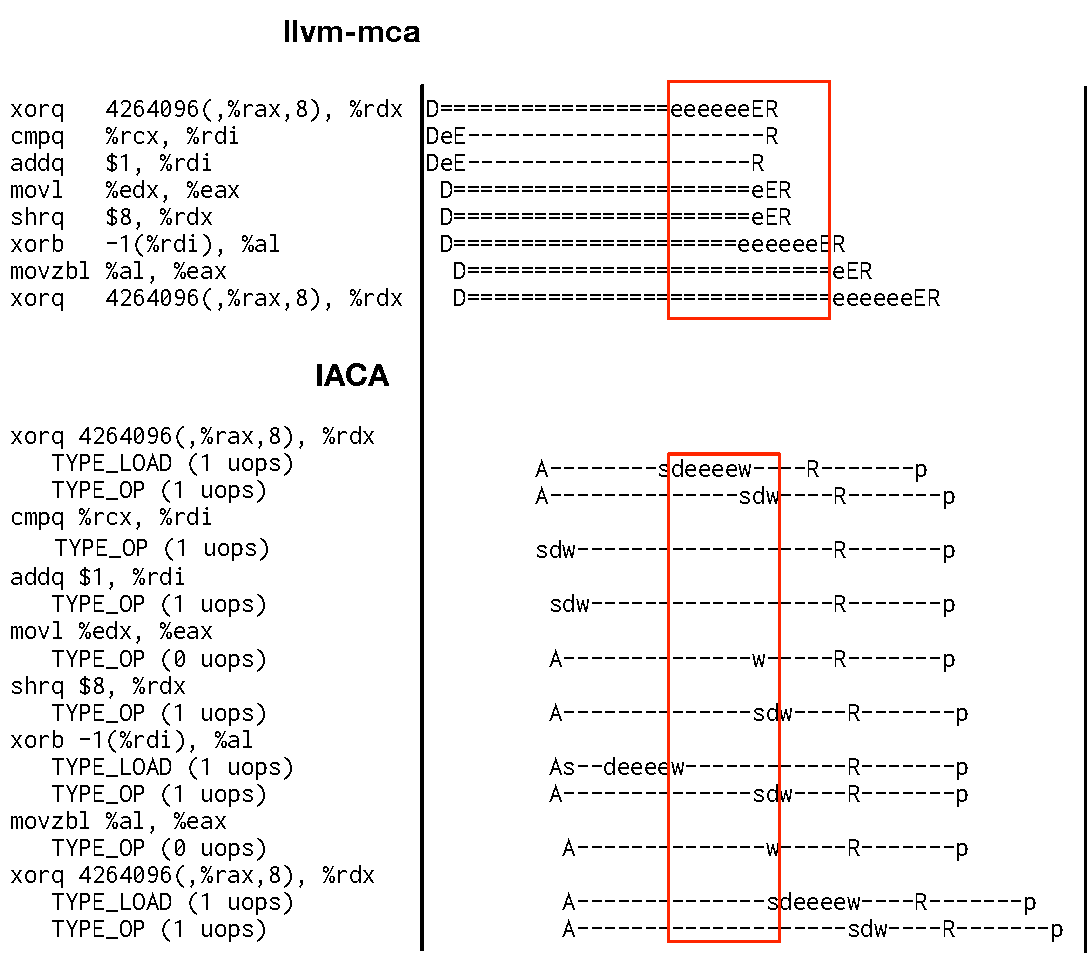
\includegraphics[width=0.95\columnwidth]{figures/scheduling.pdf}
    \caption{Schedules predicted by llvm-mca and IACA for an example basic block.
    Each red window marks the boundary of a single iteration of execution.
    The width of the windows represents the steady state throughput.
    As illustrated here, llvm-mca and IACA predicts two different schedules.
    Notice that the xorb instruction is dispatched earlier in IACA's schedules than in llvm-mca's. 
    }
    \label{tab:case-study}
\end{figure}

\begin{figure}[htbp!]
    \begin{center}
    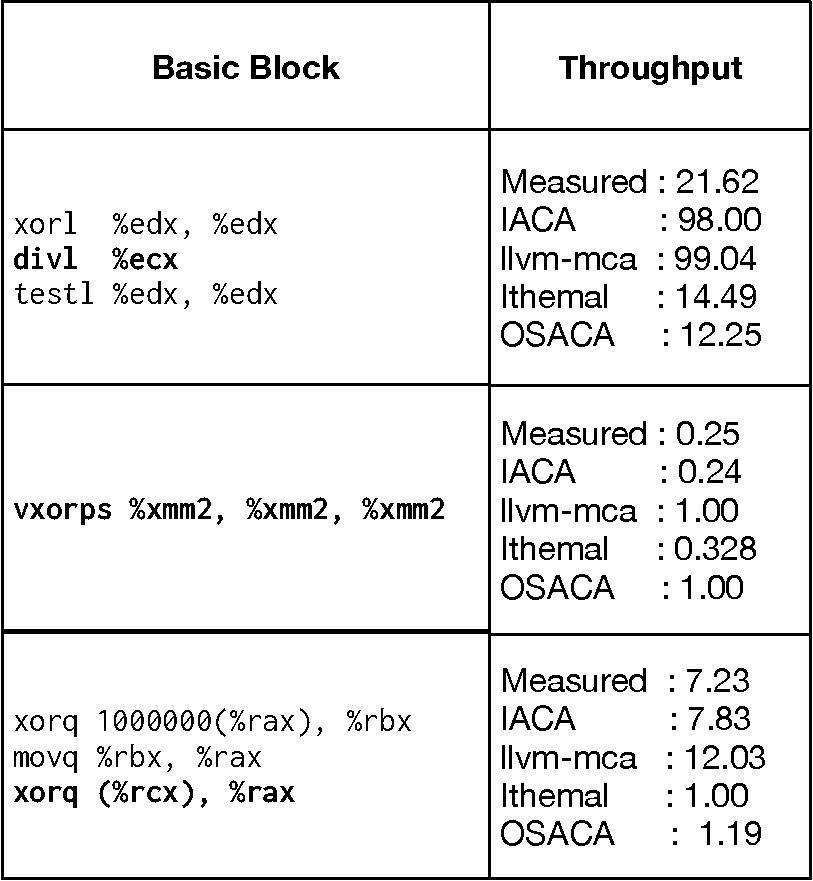
\includegraphics[width=0.7\columnwidth]{figures/interesting-examples.pdf}
    \caption{Interesting basic blocks and their inverse throughput as observed from measurements and reported by IACA, llvm-mca and OSACA (- indicates that the tool crashes while processing the basic block).}
    \label{tab:case-study}
    \label{fig:schedule}
    \end{center}
\end{figure}

\begin{comment}
\begin{table*}[t]
    \centering
    \begin{tabular}{|l|c|c|c|c|c|}
    \hline
        Basic Block & Measured & IACA & llvm-mca & Ithemal & OSACA \\
\hline
\begin{lstlisting}
xor edx, edx
div ecx
test edx, edx
\end{lstlisting}
& 21.62 & 98.00 & 99.04 & 14.49 & 12.25 \\ 
\hline

\begin{lstlisting}
vxorps	 xmm2, xmm2,  xmm2
\end{lstlisting}
& 0.25 & 0.24 & 1.00 & 0.328 & 1.00 \\ 
\hline

\begin{lstlisting}
add rdi, 1
mov eax, edx
shr rdx, 8
xor al, [rdi - 1]
movzx eax, al
xor rdx, [8*rax + 0x4110a]
cmp rdi, rcx
\end{lstlisting}
& 8.25 & 8.00 & 13.04 & 2.13 & - \\ 
\hline 
    \end{tabular} 
    \\
    ~\\
    \caption{Interesting basic blocks and their inverse throughputs as observed from measurements and reported by IACA, llvm-mca and OSACA (- indicates that the tool could not time the particular basic block).}
    \label{tab:case-study}
\end{table*}
\end{comment}